%%%%%%%%%%%%%%%%%%%%%%%%%%%%%%%%%%%%%%%%%%%%%%%%%%%%%%%%%%%%%%%%%%%%%%%%%%%%%%%%%
%																				%
%	TRABAJO:	Trabajo Final													%
%				Especialidad en Ingenier�a en Sistemas de Informaci�n			%
%																				%
%		Titulo:																	%
%																				%
%		Autores:	Julian Nonino												%
%																				%
%	Capitulo sobre Apache Storm													%	
%																				%
%	A�o: 2016																	%
%																				%
%%%%%%%%%%%%%%%%%%%%%%%%%%%%%%%%%%%%%%%%%%%%%%%%%%%%%%%%%%%%%%%%%%%%%%%%%%%%%%%%%

\chapter{Apache Storm}
\label{chapter_apache_storm}

Apache Storm es una herramienta de procesamiento de datos en tiempo real de
c�digo abierto y gratuita creada por Twitter y luego liberada en lo �rbita de
los proyectos Apache.

La finalidad de Storm es proveer un mecanismo confiable para procesamiento de
flujos de datos ilimitados, haciendo para flujos de datos (\emph{realtime
stream processing}) lo que Hadoop hace en procesamiento por lotes (\emph{batch
processing})\cite{ApacheStorm101}.

Deacuerdo a su documentaci�n, es capaz de procesar un mill�n de tuplas de datos
por segundo por nodo. Provee caracter�sticas de escalabilidad, tolerancia a
fallos, garant�as de que todos los datos ser�n procesados, etc�tera\cite{ApacheStorm101}.

Una \emph{topolog�a} de Storm consume flujos de datos, los procesa y genera
nuevos flujos de datos.

\section{Conceptos B�sicos}

	En �sta secci�n se analizar�n los conceptos b�sicos que definen a un programa
	Storm.
	
	\begin{figure}[H]
		\centering
		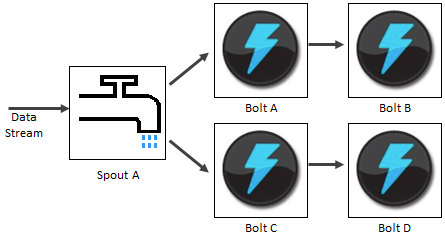
\includegraphics[width=.9\linewidth]{./marco_teorico/img/storm/topology}
	\end{figure}
	
	\subsection{\emph{Topologies} (Topolog�as)}
	
	Las \emph{topolog�as} son los contenedores de la l�gica de una aplicaci�n de
	procesamiento de datos en tiempo real. Es el an�logo a un trabajo de MapReduce
	de
	Hadoop\footnote{https://hadoop.apache.org/docs/current/hadoop-mapreduce-client/hadoop-mapreduce-client-core/MapReduceTutorial.html}.
	La diferencia principal con �stos �ltimos es que un trabajo MapReduce de
	Hadoop, eventualmente concluye mientras que las topolog�as pueden correr
	indefinidamente.
	Una topolog�a es un grafo formado por \emph{Spouts} y \emph{Bolts} conectados a
	trav�s de \emph{Stream Groupings}.
	
	\subsection{\emph{Streams} (Flujos de Datos)}
	
	\subsection{\emph{Spouts} (Tuber�as)}
	
	\subsection{\emph{Bolts} (Piezas))}

	\subsection{\emph{Streams Grouping} (Agrupamientos de Flujos de Datos)}
	
	\subsection{\emph{Tasks} (Tareas)}
	
	\subsection{\emph{Workers} (Trabajadores))}
	